\documentclass[a4j, dvipdfm]{jarticle}
\usepackage[utf8]{inputenc}     %欧文でutf-8対応にする
\usepackage[hang,small,bf]{caption}
\usepackage[subrefformat=parens]{subcaption}

\usepackage{amsmath,amssymb}    %数式
\usepackage{bm}                 %太字ベクトル
\usepackage{graphicx}           %図の挿入
\usepackage{here}               %図の[H]を使えるようにする
\usepackage{ascmac}             %枠を使う
\usepackage{physics}            %コマンドの略称を用いる
\usepackage{comment}            %コメントの使用
\usepackage{enumerate}          %箇条書きを可能に
\usepackage{url}                %urlの利用
\usepackage{listings,jvlisting}
\usepackage[dvipdfmx]{hyperref}
% \usepackage{pxjahyper}

\pagestyle{empty}
\begin{document}
{\Large コンピュータ物理学}
\hskip1zw \hfill
\underline{ 3年 \hskip2zw \hskip2zw 学籍番号: 05502231\hskip3zw 氏名  松田愛理\hskip15ex }
\vspace*{2ex}
\begin{enumerate}[問題(1)]
  \large \item オイラー法の説明\\

        オイラー法とは、一階の微分方程式
        \begin{align}
          \frac{\mathrm{d}y(t)}{\mathrm{d}t} = f(t, y)
        \end{align}
        について、ある時刻$t_n$での変化量$f(t_n, y_n)$を求めることにより時間$h$だけ進めた時の$y(t)$の値$y_{t_n +h}$を求める方法。既知の値$y(t_n+h)$についてテイラー展開が
        \begin{align}
          y(t_n + h) & = y(t_n) + h \left(\frac{\mathrm{d}y(t)}{\mathrm{d}t}\right)_{t=t_n} + \mathcal{O}(h^2) \\
                     & \simeq y(t_n) + h \left(\frac{\mathrm{d}y(t)}{\mathrm{d}t}\right)_{t=t_n}
        \end{align}
        となることから、初期値$t=t_{start}$、$y(t)=y_0$を与えることにより任意の時刻での値$y(t)$が得られる。

        \begin{figure}[H]
          \centering
          % \includegraphics[height=10cm]{}
          \caption{}
          \label{}
        \end{figure}

        \large \item 抵抗係数と角度$\theta$の関係 \\
        (1)$L$と$\theta$の関係性を求める。質量$m$、抵抗係数$b$、初速度$v_0$の値にはそれぞれ$m=0.1$、$b=0.1$、$v_0=100/3.6$の値を用いた。結果のグラフは図\ref{L_theta}の通りとなった。

        \begin{figure}[H]
          \centering
          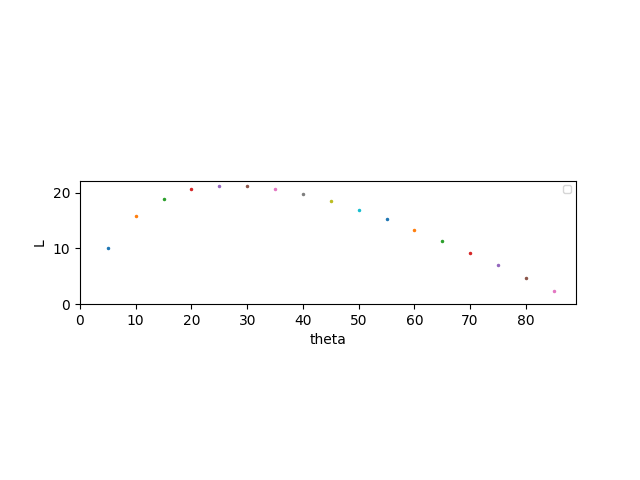
\includegraphics[height=5cm]{pic/related_theta_L.png}
          \caption{到達距離$L$と$\theta$の関係}
          \label{L_theta}
        \end{figure}

        (2)最大到達距離$L_{max}$とその時の角度$\theta$について
        次に、最大到達距離$L_max$の時の放射角度$\theta_max$と抵抗係数$b/m$の関係を計算した。図\ref{change_bm}は抵抗係数$b/m$を変更したときの到達距離$L$と放射角度$\theta$を表している。
        \begin{figure}[H]
          \centering
          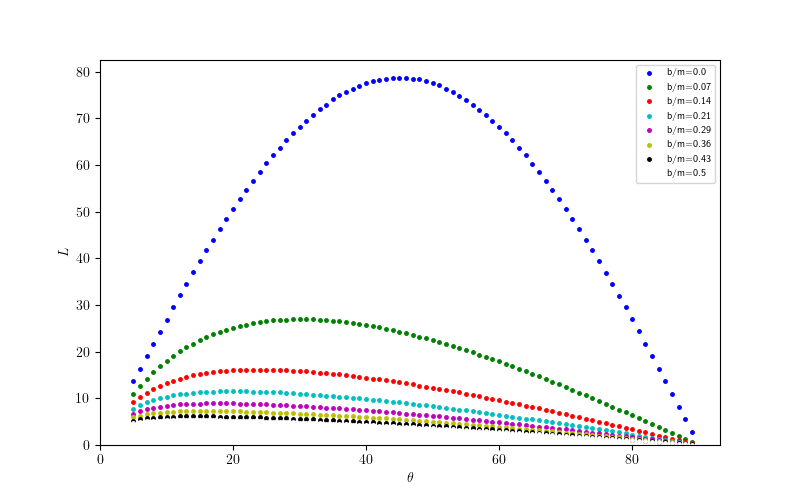
\includegraphics[width=12cm]{pic/change_bm.png}
          \caption{抵抗係数$b/m$を変えた時の到達距離$L$と角度$\theta$の関係}
          \label{change_bm}
        \end{figure}

        図\ref{change_bm}から、抵抗が大きくなるに従って最大到達距離が小さくなると同時にのそのときの放射角も小さくなっている(だんだん凸部が左に寄ったグラフになっている)ことが分かる。実際に、この最大到達距離を示す放射角度$\theta_max$と抵抗係数$b/m$の関係を図示すると、図\ref{theta_max}の通りになった。

        \begin{figure}[H]
          \centering
          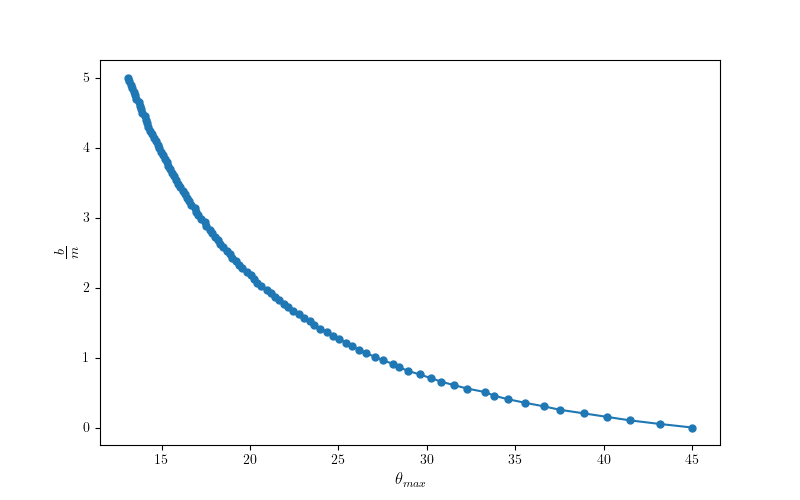
\includegraphics[width=12cm]{pic/related_theta_bm.png}
          \caption{}
          \label{theta_max}
        \end{figure}
        図\ref{theta_max}の結果は抵抗係数$b/m=0$の時に$\theta_max=45$[°]、抵抗係数が無限大で十分大きくなると$\theta_max=0$に近づき、直感的な解釈と合致する。


        \begin{flushright}
          \href{https://github.com/eri61/computer_physics/blob/1336fc7c853c9eda9e7e32c47d7df82ef45bb469/report1/code/report01_05502231Matsuda.ipynb}{ノートブック}
        \end{flushright}
\end{enumerate}
\end{document}